\documentclass{article}
\usepackage[final]{neurips_2024}
\usepackage[T1]{fontenc}    
\usepackage{hyperref}       
\usepackage{url}            
\usepackage{booktabs}       
\usepackage{amsfonts}       
\usepackage{nicefrac}       
\usepackage{microtype}      
\usepackage{xcolor}         
\usepackage{graphicx}   
\usepackage{amsmath}

\setcitestyle{numbers}

\title{COMP 579 Final Project Report: Reinforcement Learning for Ms. Pac-Man}

\author{
  Ivy Hu \\
  nanqing.hu@mail.mcgill.ca \\
  Department of Computer Science\\
  McGill University
  \And
  Simon Li \\
  xi.yang.li@mcgill.ca\\
  Department of Electrical Eng.\\
  McGill University
  \And
  Kenza Bellebouir\\
  kenza.bellebouir@mail.mcgill.ca\\
  Department of Computer Science\\
  McGill University
}

\begin{document}

\maketitle

\section{Introduction}

Deep reinforcement learning (RL) has achieved remarkable success in solving a variety of challenging sequential decision-making tasks, particularly in high-dimensional environments such as Atari 2600 games \cite{mnih2015human}. These games, accessible through the Arcade Learning Environment (ALE) \cite{ale}, provide an ideal testbed for evaluating RL algorithms due to their complex dynamics, partial observability, sparse rewards, and the need for both short-term reactivity and long-term planning. Among these, the game \textit{Ms. Pac-Man} stands out as a particularly difficult benchmark: it features stochastic ghost behavior, multiple strategies for survival and scoring, and a visually rich input space, making it an ideal environment for testing the robustness and scalability of RL algorithms.

In this project, we focus on evaluating and analyzing two prominent families of RL algorithms: value-based methods, represented by Rainbow DQN \cite{hessel2018rainbow}, and policy-based methods, represented by Proximal Policy Optimization (PPO) \cite{schulman2017proximal}. Rainbow DQN is a state-of-the-art enhancement of the classic Deep Q-Network (DQN), combining multiple algorithmic improvements into a single agent. These include double Q-learning, dueling network architecture, prioritized experience replay, multi-step bootstrapping, noisy networks for exploration, and distributional value representation. PPO, on the other hand, is a widely used policy gradient method known for its training stability and simplicity.

Our primary goal is to conduct a comprehensive empirical study of these two algorithms in the \texttt{MsPacman-v0} environment from OpenAI Gym. We go beyond standard benchmarking by performing an ablation study on the Rainbow DQN architecture to quantify the impact of its individual components. Specifically, we evaluate the performance impact of removing prioritized replay, noisy linear layers, and multi-step returns. Additionally, we examine the robustness of trained agents by altering the visual input through color perturbations. This form of analysis helps assess the generalization capabilities of agents trained in visually consistent environments when exposed to minor domain shifts.

We also investigate the role of hyperparameter selection in performance, conducting targeted hyperparameter sweeps for both Rainbow DQN and PPO to identify high-performing configurations. Our experiments measure performance in terms of average episode return, sample efficiency, training stability, and robustness to visual perturbation.

\textbf{Our contributions are as follows:}
\begin{itemize}
    \item We implement and train Rainbow DQN and PPO agents in the Ms. Pac-Man environment, comparing their overall learning performance and stability.
    \item We perform an ablation study on Rainbow DQN, isolating the effects of prioritized replay, noisy exploration, and multi-step returns.
    \item We evaluate the robustness of trained agents by modifying the visual appearance of game frames and analyzing their performance in these shifted domains.
    \item We present insights into the sensitivity of both algorithms to hyperparameter choices, identifying factors critical to successful training.
\end{itemize}

Through these contributions, we aim to better understand the internal mechanics of Rainbow DQN, its strengths and limitations in complex visual tasks, and how it compares to PPO in both standard and perturbed conditions. The findings of this project provide a practical perspective on designing and evaluating RL algorithms in visually diverse environments, offering guidance for future work in generalization and robustness in deep RL.

\section{Background}

\subsection{Reinforcement Learning and Markov Decision Processes}

Reinforcement Learning (RL) is a framework for sequential decision-making where an agent interacts with an environment to learn a policy that maximizes cumulative reward. The problem is commonly formalized as a Markov Decision Process (MDP), defined by the tuple $(\mathcal{S}, \mathcal{A}, \mathcal{P}, \mathcal{R}, \gamma)$, where $\mathcal{S}$ is the set of states, $\mathcal{A}$ the set of actions, $\mathcal{P}(s'|s, a)$ the transition dynamics, $\mathcal{R}(s, a)$ the reward function, and $\gamma \in [0, 1)$ the discount factor. At each timestep, the agent observes a state $s \in \mathcal{S}$, selects an action $a \in \mathcal{A}$, receives a scalar reward $r$, and transitions to a new state $s'$. The goal is to learn a policy $\pi(a|s)$ that maximizes the expected return $\mathbb{E}[\sum_t \gamma^t r_t]$.

\subsection{The Ms. Pac-Man Environment}

The \texttt{MsPacman-v0} environment from the Arcade Learning Environment (ALE) \cite{ale} presents a complex MDP characterized by a high-dimensional visual state space and long-horizon planning requirements. Observations are $210 \times 160 \times 3$ RGB images, which we preprocess into $84 \times 84$ grayscale frames. The action space is discrete, consisting of directional inputs and a no-op action. Rewards are sparse and consist of: +10 for collecting pellets, +200 for eating a ghost with a power pellet, and a time-penalty of –1 per step. Episodes terminate after the agent loses all three lives.

This environment poses several RL-specific challenges:
\begin{itemize}
    \item \textbf{Partial observability:} The game state is partially observable from pixel inputs, and ghost movement patterns are not fully predictable.
    \item \textbf{Sparse and delayed rewards:} Feedback is infrequent and often delayed, making credit assignment non-trivial.
    \item \textbf{Lack of dense reward shaping:} There is no built-in intermediate reward signal for beneficial behaviors like path planning or threat avoidance.
\end{itemize}

\subsection{Deep Q-Networks and Rainbow DQN}

The Deep Q-Network (DQN) algorithm \cite{mnih2015human} approximates the action-value function $Q(s, a)$ using a deep convolutional neural network trained with the Bellman error. DQN was the first RL algorithm to achieve human-level performance in many Atari games directly from pixel inputs.

Rainbow DQN \cite{hessel2018rainbow} enhances DQN by integrating several complementary improvements:
\begin{itemize}
    \item \textbf{Double Q-learning} reduces overestimation bias by decoupling action selection from target value estimation.
    \item \textbf{Dueling network architecture} decomposes $Q(s, a)$ into a state-value function $V(s)$ and an advantage function $A(s, a)$ to better estimate the importance of each action.
    \item \textbf{Prioritized experience replay} samples more important transitions with higher probability, improving sample efficiency.
    \item \textbf{Noisy Networks} add learned parametric noise to weights in fully connected layers to encourage more efficient exploration.
    \item \textbf{Multi-step returns} enable faster propagation of reward signals by using $n$-step bootstrapped targets.
    \item \textbf{Distributional RL (C51)} models the full distribution over future returns instead of just the expectation, using a fixed discrete support of return values and a softmax-based categorical projection.
\end{itemize}

These components jointly aim to improve the stability, learning speed, and final performance of the agent across diverse environments.

\subsection{Proximal Policy Optimization (PPO)}

Proximal Policy Optimization (PPO) \cite{schulman2017proximal} is a policy-gradient method that directly optimizes the expected return by sampling trajectories and computing gradient estimates with respect to the policy parameters. PPO uses a clipped surrogate objective to avoid large policy updates, which can destabilize training. The objective function is defined as:
\[
L^{\text{CLIP}}(\theta) = \mathbb{E}_t \left[ \min \left( r_t(\theta) \hat{A}_t, \text{clip}(r_t(\theta), 1 - \epsilon, 1 + \epsilon) \hat{A}_t \right) \right],
\]
where $r_t(\theta)$ is the probability ratio between the new and old policies, and $\hat{A}_t$ is an estimator of the advantage function. PPO is widely used due to its simplicity, generality, and empirical robustness.

\subsection{Challenges in Evaluation}

Evaluating RL algorithms in environments like Ms. Pac-Man involves several challenges beyond simply achieving a high score:
\begin{itemize}
    \item \textbf{Training stability:} RL training can be unstable due to non-stationarity, bootstrapping errors, and sensitivity to hyperparameters.
    \item \textbf{Sample efficiency:} Especially in visual domains, training can require millions of environment frames; algorithms that learn faster are preferred.
    \item \textbf{Generalization:} Agents trained on a specific visual environment often fail when exposed to even minor changes. Zhang et al. \cite{zhang2020investigation} showed that Rainbow DQN fails under simple color transformations, motivating our experiments on visual robustness.
\end{itemize}

\subsection{Related Approaches in Ms. Pac-Man}

Prior research has explored enhancements to standard RL in Ms. Pac-Man. Toromanoff et al. \cite{toromanoff2019deep} introduced a memory-augmented agent combining CNNs with RNNs to improve partial observability, showing performance that exceeded DQN by 2x. Hybrid planning-RL methods, such as those by Pieters et al. \cite{pieters2016monte}, have applied Monte Carlo Tree Search (MCTS) for power pellet usage, though these rely on handcrafted state features. In contrast, our work focuses on pure pixel-based learning without external knowledge. Our experiments also extend visual generalization analysis by explicitly testing color perturbations during evaluation.

\section{Methodology}

\subsection{Environment}

We evaluate our agents using the \texttt{MsPacman-v0} environment from OpenAI Gym, built on the Arcade Learning Environment (ALE) \cite{ale}. The environment provides raw RGB frames of size $210 \times 160 \times 3$, which we preprocess into $84 \times 84$ grayscale or colored images, normalized to the $[0, 1]$ range. To capture temporal dynamics, we stack the last 4 frames as input to the agent, providing a simple form of memory. The action space contains 9 discrete actions including the 4 cardinal directions, 4 diagonals, and a no-op. The reward structure is sparse and native to the game: +10 for collecting pellets, +200 for eating ghosts after consuming a power pellet, and –1 as a per-step time penalty. Episodes terminate after the agent loses all 3 lives.

\subsection{Preprocessing}

We use two preprocessing pipelines in our experiments:

\begin{itemize}
    \item \textbf{Baseline Preprocessing:} RGB frames are converted to grayscale and resized to $84 \times 84$ pixels using bilinear interpolation. Pixel values are normalized and stacked across 4 timesteps.
    
    \item \textbf{Color Perturbation Preprocessing:} To evaluate robustness, we introduce a custom wrapper \texttt{ColorPreprocessFrame}, which first converts each frame to grayscale and then applies a color tint or OpenCV colormap. The output is a 3-channel RGB image. Tint variants include red, green, and blue scaling, while colormap variants include \texttt{cv2.COLORMAP\_JET}, among others. This allows us to test whether agents trained in standard conditions can generalize under visually altered but semantically identical states.
\end{itemize}

\subsection{Model Architectures}

\paragraph{Rainbow DQN.}
We implement the full Rainbow DQN \cite{hessel2018rainbow} architecture, combining several enhancements over the original DQN \cite{mnih2015human}:
\begin{itemize}
    \item A convolutional backbone with three layers (32, 64, 64 filters) followed by a flattening layer;
    \item A dueling network head with separate value and advantage streams;
    \item NoisyLinear layers for exploration, with initial standard deviation $\sigma=0.017$;
    \item A distributional output using 51 atoms over the fixed value range $[-10, 10]$;
    \item Prioritized experience replay with $\alpha = 0.6$ and $\beta$ annealed from 0.4 to 1.0;
    \item Multi-step learning with $n = 3$.
\end{itemize}
The target network is updated every 1,000 environment steps. The model is trained using the Adam optimizer with a learning rate of $1 \times 10^{-4}$.

\paragraph{Proximal Policy Optimization (PPO).}
Our PPO implementation follows the standard actor-critic design, using a shared convolutional feature extractor with the same architecture as Rainbow DQN, followed by a 512-unit fully connected layer. The actor and critic heads branch from this shared backbone. We optimize the clipped surrogate objective with $\epsilon = 0.1$ and use Generalized Advantage Estimation (GAE) with $\lambda = 0.95$. Training is conducted using a batch size of 32, and a learning rate of $2.5 \times 10^{-4}$, for 1000 updates using 256-step rollouts, totaling 256,000 environment steps.

\subsection{Training Details}

Both agents are trained using frame-stacked observations and the Adam optimizer. The Rainbow DQN agent is trained for 30,000 to 50,000 frames per experimental setting, while PPO is trained for 1000 steps due to its on-policy nature. We use a single reproducibility seed (357) across all experiments due to time constraints and limited compute. Each training run is followed by an evaluation phase using the same environment configuration, without exploration noise.

Training and evaluation were conducted on a for the ablation and color studies were conducted on an NVIDIA RTX 3080 laptop, while the hyperparameter studies were done on a mac notebook, with end-to-end training time ranging from 2 to 5 hours depending on the experiment.

\subsection{Evaluation Protocol}

Our evaluation is based on a fixed frame budget for each agent, after which performance is measured in terms of:

\begin{itemize}
    \item \textbf{Average episode return:} Cumulative score achieved per episode during training.
    \item \textbf{Final performance:} Episode return after training concludes, shown in our results figures.
\end{itemize}

\section{Results and Discussion}

\subsection{Rainbow DQN vs. PPO: Learning Performance}

Figure~\ref{fig:ppo_vs_rainbow} presents the training performance of our PPO and Rainbow DQN agents in the \texttt{MsPacman-v0} environment. While neither agent reaches expert-level performance within the limited frame budget, we observe several qualitative and quantitative differences between the two learning dynamics.

The PPO agent (top) exhibits highly variable performance throughout the training process. Initially, it converges to a moderately stable reward range of 200–300 after approximately 250 updates (equivalent to $\sim$64,000 frames). However, beyond update 600, performance appears to degrade significantly, with frequent fluctuations and occasional spikes. This instability could stem from on-policy sampling noise or suboptimal hyperparameter tuning. Despite this, PPO demonstrates the ability to learn basic survival and pellet-collection strategies early in training.

In contrast, the Rainbow DQN agent (bottom) shows a clearer upward trajectory over the course of training. Reward variability is also high, but we observe several distinct peaks exceeding 1000 and even 2000 points, indicating that the agent has discovered higher-reward behaviors (e.g., efficient pellet clearing or ghost chasing). The learning curve is less smooth but shows better long-term reward potential. This aligns with Rainbow’s design as a more sample-efficient value-based method that benefits from prioritized replay and distributional learning.

\begin{figure}[h]
    \centering
    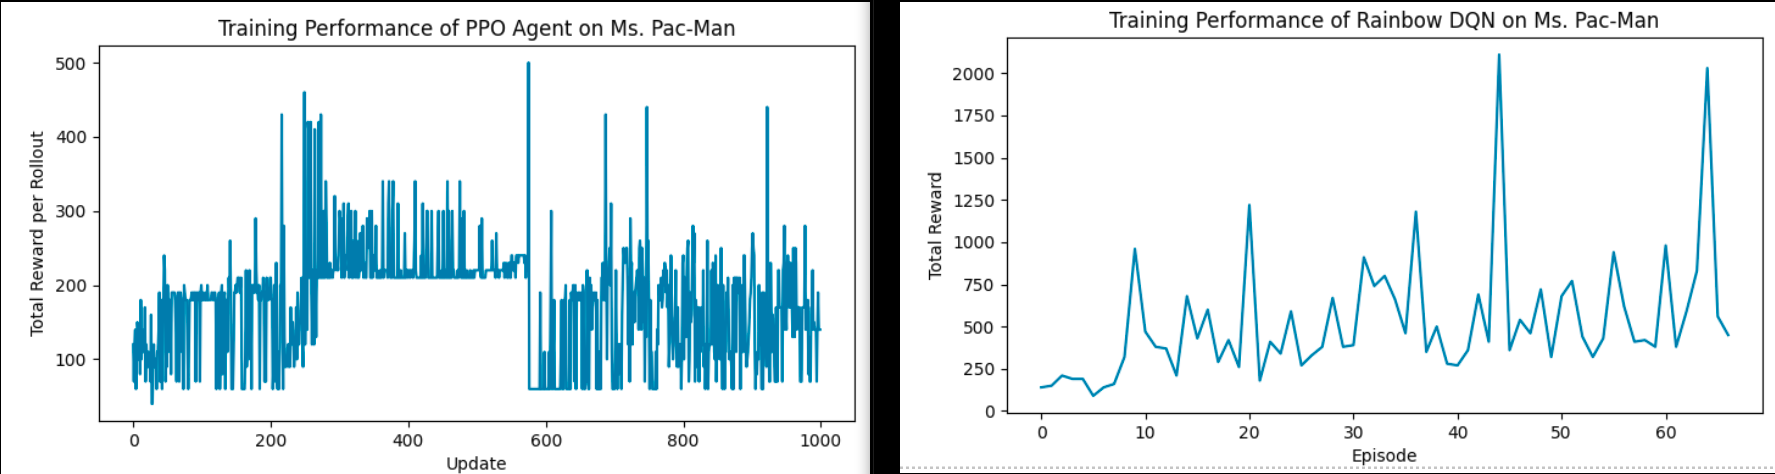
\includegraphics[width=0.85\linewidth]{rainbow_vs_ppo.png}
    \caption{Left: Training performance of PPO agent (total reward per 256-step rollout); Right: Training performance of Rainbow DQN agent (total reward per episode).}
    \label{fig:ppo_vs_rainbow}
\end{figure}

\subsection{Interpretation and Comparative Insights}

Both agents show signs of early learning, but Rainbow DQN achieves significantly higher peak rewards than PPO. This suggests that value-based methods, particularly those enhanced by Rainbow’s extensions (e.g., prioritized replay, noisy exploration, and multi-step targets), may be more effective at discovering high-reward strategies in sparse-reward, long-horizon environments like Ms. Pac-Man.

However, the volatility in both plots indicates that neither agent has fully stabilized. PPO’s reward collapse in later updates highlights the sensitivity of policy gradient methods to training hyperparameters and the challenges of on-policy learning in high-dimensional settings. Conversely, Rainbow’s high variance suggests that better reward shaping, more training time, or additional architectural tuning (e.g., learning rate, replay buffer size) might be needed to achieve consistent gains.

In summary, Rainbow DQN shows greater promise in this environment under the current constraints, exhibiting higher peak performance and a stronger upward trend. PPO’s learning is less consistent, though its earlier convergence and training stability in the initial phase suggest it may benefit from a more extensive rollout horizon or different GAE parameters.

\subsection{Rainbow DQN Ablation Study}

To better understand the contribution of individual components within the Rainbow DQN architecture, we conducted a series of ablation experiments. Specifically, we evaluated three reduced versions of Rainbow:
\begin{itemize}
    \item \textbf{nstep1:} Multi-step returns are disabled by setting $n=1$ (i.e., single-step targets).
    \item \textbf{no\_prior:} Prioritized replay is replaced with uniform sampling.
    \item \textbf{no\_noisy:} NoisyLinear layers are replaced with standard linear layers, disabling learned exploration.
\end{itemize}

Figure~\ref{fig:rainbow_ablation} shows the training performance of the full Rainbow agent compared to each ablation over 45 episodes. While all variants remain within a similar average performance range (200–700 points), some key trends emerge.

First, we observe that the \textbf{full Rainbow} configuration occasionally achieves significantly higher rewards (e.g., a spike around episode 7 and another at episode 20), suggesting that the combined effects of prioritized replay, multi-step returns, and noisy exploration facilitate effective strategy discovery. However, these peaks are interspersed with episodes of mediocre performance, indicating instability during early training.

The \textbf{no\_prior} variant performs comparably well in later episodes, even outperforming full Rainbow for sustained periods after episode 25. This suggests that while prioritized replay can accelerate early learning, it may not be essential for eventual policy quality—at least under limited training conditions.

Interestingly, the \textbf{no\_noisy} agent shows stronger improvement toward the end of training compared to the baseline, reaching scores above 1000 in multiple episodes. This indicates that deterministic policies may offer better stability in this environment, though they may initially explore less effectively.

Finally, the \textbf{nstep1} variant consistently underperforms across the entire training window. This confirms the importance of multi-step bootstrapping for sparse reward propagation in long-horizon environments like Ms. Pac-Man.

\begin{figure}[h]
    \centering
    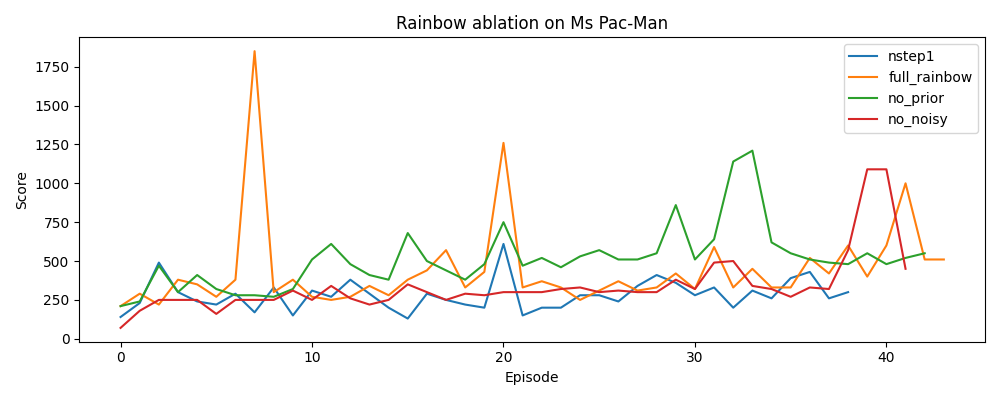
\includegraphics[width=\linewidth]{rainbow_ablation.png}
    \caption{Training performance of Rainbow DQN and ablated variants on Ms. Pac-Man. Each line shows episode rewards for a different configuration.}
    \label{fig:rainbow_ablation}
\end{figure}

\subsubsection*{Summary of Findings}
\begin{itemize}
    \item Multi-step returns ($n > 1$) are critical for performance in sparse-reward settings.
    \item Prioritized replay improves early exploration, but may be less important for long-term policy success.
    \item Noisy exploration accelerates early learning but may introduce instability; deterministic networks (no\_noisy) can still perform well.
\end{itemize}

These insights reinforce the utility of Rainbow’s component-wise enhancements while also suggesting that certain components, like prioritized replay, may be omitted in resource-constrained deployments without catastrophic performance loss.

\bibliographystyle{plain}
\bibliography{references}

\end{document}
